\documentclass[../598comp.tex]{subfiles}

\graphicspath{ {./lectures/images/}{./images/} }

\date{05-20}

\begin{document}

\section{05-20}

Proving pumping lemma we used the way that DFA has finitely many states. But the
size of the stack can be infinite. Instead we use the fact that a grammar for a
CFL has only finitely many variables.

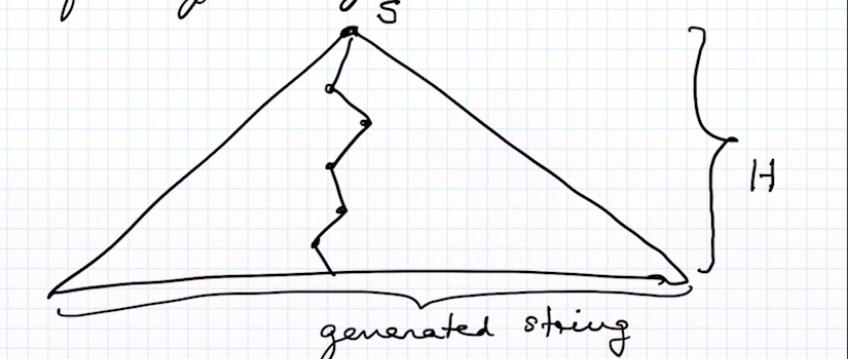
\includegraphics[width=\textwidth]{parse_tree_example}

Height of parse tree increases less quickly than the length of the word. For a
long enough word, $H > \#$ of non terminals in the grammar.

This means that at some point there has to be a repeated non-terminal.

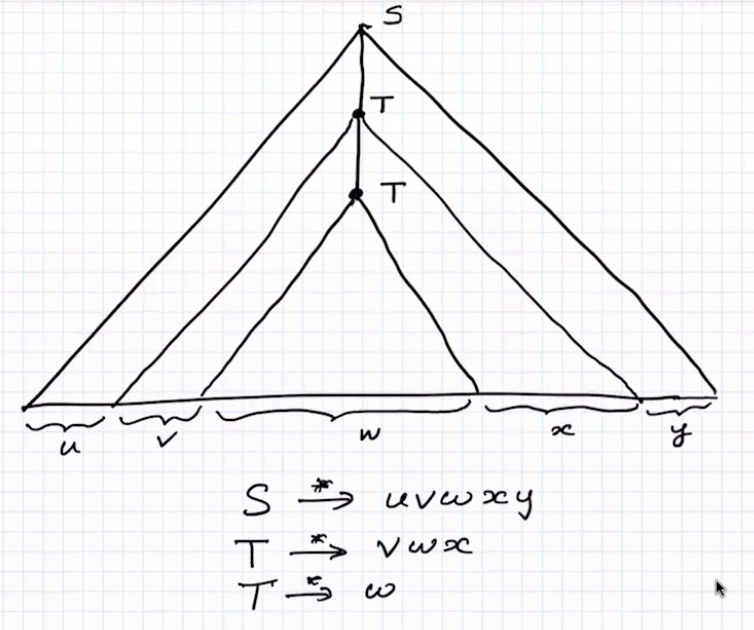
\includegraphics[width=\textwidth/4*3]{parse_tree_example2}

It is not possible that both $v$ and $x$ are empty. This is true if we assume
Noam Chomsky form. But then we can change the second $T$ into generating $vwx$
which would mean thta $uv^2wx^2y \in L$. And you can do this again
which would mean $uv^3wx^3y \in L$. We conclude that
\begin{gather*}
  \forall i \geq 0 \ uv^iwx^i \in L
\end{gather*}

\begin{lemma}[Pumping Lemma for Context Free Languages]
  \begin{gather*}
    \forall CFL, L, \ \exists p > 0 \\
    \forall s \in L \ |s| \geq p \\
    \exists u, v, w, x, y \in \Sigma^* \ \text{s.t.} \ s = uvwxy, \ |vx| > 0 \
    , |vwx| \leq p \\
    \forall i \geq 0, \ uv^iwx^iy \in L
  \end{gather*}
  No longer guaranteeing that is happens early on in the string.
\end{lemma}

\begin{lemma}[Contrapositive of Pumping Lemma for Context Free Languages]
  Fix some language $L$.
  \begin{gather*}
    \forall p > 0, \ \exists s \in L, \ |s| \geq p \\
    \forall u, v, w, x, y \in \Sigma^* \\
    s = uvwxy, \ |vx| > 0, |vwx| \leq p \\
    \exists i \geq 0, \ uv^iwx^iy \notin L \\
    \Rightarrow L \ \text{is not context free}
  \end{gather*}
\end{lemma}

\begin{example}
  $L = \{a^nb^na^n \ | n \geq 0\}$.
  \begin{enumerate}
  \item 
    Demon chooses $p$
  \item
    We choose $a^pb^pa^p$.
  \item
    Possibilities for $uvwxy$.
    \begin{enumerate}
    \item 
      If $v$ or $x$ stradles a block boundary, the demon loses with $i = 2$
      because the $a$'s and $b$'s will be out of order.
    \item
      If $v$ and $x$ both contain only $a$'s they must be in the same block.
      The demon loses with $i = 2$ because blocks will no longer be of the same size.
    \item
      If $v$ and $x$ contain only $b$'s, the demon loses with $i = 2$ because
      the $b$ block is too long.
    \item
      If $v$ contains only $a$'s and $x$ contains only $b$'s, then demon loses
      with $i = 2$ because the untouched block will be of different length.
    \end{enumerate}
  \item
    Therefore the language is not context free because we have a winning strategy.
  \end{enumerate}
\end{example}

\begin{example}
  $L = \{a^nb^n \ | \ n \geq 0\}$. In the regular case, the $y$ consists of only
  $a$'s so we win. But now in the context free case, there isn't a winning strategy.
  
  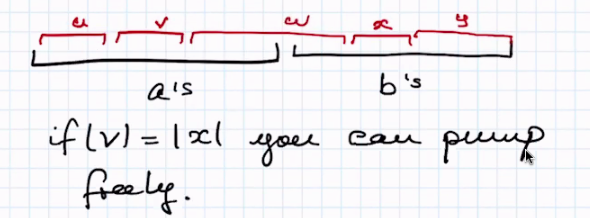
\includegraphics[width=\textwidth]{context_pumping_example}
\end{example}

\begin{example}
  $L = \{a^{i + j}b^{j + k}c^{i + k} \ | \ i, j, k \geq 0\}$. Try to recognize instictively whether or not the language is context free before proving it.

  This is context free! Trying to reason about why. $i + j$ is unbounded, but
  the stack is also unbounded. A lot more tricky to check CFGness.

  Exercise: Cook up a CFG for this.
\end{example}

\begin{example}
  $|\Sigma| \geq 2$. $L = \{ww \ | \ w \in \Sigma^*\}, \ L' = \{ww^{REV} \ | \ w
  \in \Sigma^*\}$. The first is not context free while the second is. The first
  is not possible because it's difficult to check if the strings are the same.
  The second is context free because the stack is good for checking the reversed string.
\end{example}

\begin{fact}
  If $L$ is CF and $R$ is regular, then $L \cap R$ is a CFL.
\end{fact}

\begin{example}
  $L = \{ww \ | \ w \in \Sigma^*\}$. We use $R = a^*b^*a^*b^*$ and show $L \cap a^*b^*a^*b^*$ is not a CFL so $L$
  cannot be a CFL.

  \begin{enumerate}
  \item 
    Demon chooses $p$.
  \item
    We choose $a^pb^pa^pb^p$.
  \item
    Possibilities for $uvwxy$.
    \begin{enumerate}
    \item 
      If $v, x$ straddle block boundaries, the demon will lose
    \item
      If $v, x$ are in the same block the demon loses because words aren't the
      same length.
    \item
      $v$ and $x$ have to be in consecutive blocks because of the bounded size
      of $vwx$. Note that the first copy of $w$ starts with $a$ so the second
      word cannot start with $b$. Also that the second copy ends with $b$ so the
      first copy must end with $b$. So the boundary between 2 copies of $w$ has
      to be at the end of the 2nd block. So although the two words could be the
      same size, they won't be the same words.
    \end{enumerate}
  \item
    Therefore there is a strategy to always beat the devil so the language is
    not context free.
  \end{enumerate}
\end{example}

\begin{example}
  $L = \{0^i1^j \ | \ j = i^2\}$. This is not a CFL.

  Let $A$ be the adversary and $I$ be us.
  \begin{enumerate}
  \item 
    $A \to p$
  \item
    $I \to 0^p1^{p^2}$
  \item
    $A \to uvwxy = 0^p1^{p^2}, \ |vwx| \leq p, \ |vw| > 0$.
  \item
    $I \to $ case analysis
    \begin{enumerate}
    \item 
      $vwx$ all zeros pick any $i \neq 1$.
    \item
      $vwx$ all ones, pick any $i \neq 1$.
    \item
      $v, x$ straddles the boundary, $i = 2$ gives $0$'s and $1$'s out of order.
    \item
      $v$ is all zeros and $x$ is all ones. We pick $i = 2$. Only non trivial
      case is when $|v| = m > 0, \ |x| = q > 0$. Pumping to $i = 2$ gives $0^{p
        + m}1^{p^2 + q}$. How do we know that $(p + m)^2 \neq p^2 + q$?
      \begin{gather*}
        (p + m)^2 = p^2 + 2pm + m^2 \\
        2pm > p \Rightarrow 2pm + m^2 > p > q \Rightarrow p^2 + 2pm + m^2 > p^2
        + q
      \end{gather*}
    \end{enumerate}
  \end{enumerate}
\end{example}

\begin{example}
  $L = \{a^q \ | \ q \ \text{a prime} \}$. Even with a stack you cannot check this.
  \begin{enumerate}
  \item 
    $A \to p$
  \item
    $I \to a^q \ | q > p$, prime
  \item
    $A \to uvwxy \ \text{s.t.} \ |uvwxy| = q, \ |vwx| \leq p, \ |vw| > 0$.
  \item
    Let $vx = r > 0$. Let $i = q + 1$. Then $|uv^iwx^iy| = q + qr = q(1 + r)$.
    Can't be a prime because it's the product of two number where each is
    greater than 1.
  \end{enumerate}
\end{example}

\begin{theorem}
  Over a one-letter alphabet a language is context-free if and only if it is regular.
\end{theorem}

\begin{example}
  $L = \{a^{2^n} \mid n \geq 0\}$ is not a CFL. We showed that this language was
  not regular.
\end{example}

\begin{exercise}
  $L = \{a^kb^jc^k \mid 0 < i < j < k\}$. Show that this is not a CFL.
\end{exercise}

\begin{definition}[DPDA]
  PDA's feature non determinism. This cannot be eliminated so DPDA's are strictly
  less powerful than PDA's.

  If a CFL can be recognized by a DPDA we call it a Deterministic CFL. All modern
  languages are DCFL's. This makes things fast.

  DPDA is a DFA with a stack.
\end{definition}

\begin{fact}
  DCFL's are closed under complement and therefore under intersection.
\end{fact}

\begin{example}
  $L = \{ww \mid w \in \Sigma^*\}, \ |\Sigma| \geq 2$. This is not a CFL, but
  $\ol{L}$ \ul{is} a CFL.

  $\ol{L}$ an be recognized by a PDA. What is in $\ol{L}$.
  \begin{enumerate}
  \item 
    Strings of odd length.
  \item
    Might be even length. Then it can be written as concatenation of two equal
    length words where the words are not equal to one another. $|w_1| = |w_2|$
    but $w_1 \neq w_2$. Two words are not the same if there exists $i$ such that
    $w_1[i] \neq w_2[i]$.
  \end{enumerate}
  Crucial difference is that instead of checking every position, you only have
  to guess one position. If there is an existing path, it works.

  The idea is guess where $i$ is and guess where the middle of the word is. It
  is okay that this $i$ is unbounded because of the non determinism.

  How the PDA works:

  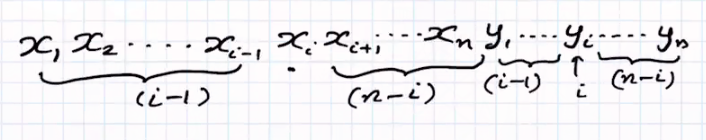
\includegraphics[width=\textwidth]{pda_word_example6.png}

  Push $x_1 \dots x_{i - 1}$ onto the stack. Then remember what $x_i$ is in the
  state. Start popping the stack until it is empty. Then start pushing letters
  onto the stack. It guesses where $y_i$ is. It looks at $y_i$ and compares it
  with $x_i$. It then pops the stack as it reads the remeaining letters. If the
  stack is empty at the end then $x_i$ and $y_i$ are indeed at the right positions.

  $(i - 1)$ symbols on the stack. $(n - i) + (i - 1) = n - 1$ between $x_i$ and $y_i$.

  After checking $y_i$ there are $(n - i)$ letters on the stack. This exactly
  matches the $(n - i)$ letters after $y_i$.

  Key point is didn't have to look at all the symbols, but used them to count.
\end{example}

\begin{example}
  Equivalent CFG for $\ol{L}$. Let $V = \{S, A, B, C\}, \ \Sigma = \{a, b\}$.
  \begin{gather*}
    S \to 
  \end{gather*}
  $A$ produces odd length words with $a$ in the middle.

  $B$ produces odd length words with $b$ in the middle.

  $S \to AB$ ultimately generates $xay \ ubv$. $n = |x| = |y|$ and $m = |u| = |v|$.

  There is guaranteed to be \ul{one} place where the corresponding positions are
  not the same.
\end{example}

Coming up. 
\begin{enumerate}
\item 
  Thursday. Concept of computability. Models of computation. Unsolvable problems. CE functions. Dovetailing.
\item
  Monday. Reduction.
\item
  Tuesday. FOC.
\item
  Wednesday. Lambda-calculus.
\item
  Thursday. Godel's Theorem. Recursion Theorem.
\end{enumerate}

\end{document}